\documentclass{article}
\usepackage{pgfplots}
\pgfplotsset{compat=1.18}

\begin{document}
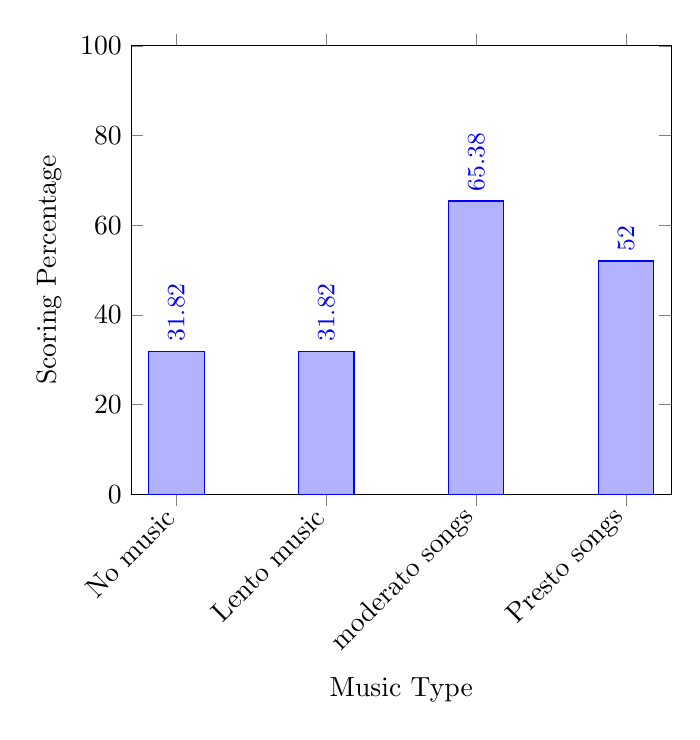
\begin{tikzpicture}
\begin{axis}[
    ybar,
    bar width=20pt,
    xlabel={Music Type},
    ylabel={Scoring Percentage},
    x tick label style={rotate=45, anchor=east},
    ymin=0,
    ymax=100,
    xtick=data,
    xticklabels={No music, Lento music, moderato songs, Presto songs},
    nodes near coords,
    every node near coord/.append style={font=\small, rotate=90, anchor=west},
    nodes near coords align={vertical},
]
\addplot coordinates {(1, 31.82) (2, 31.82) (3, 65.38) (4, 52.0)};
\end{axis}
\end{tikzpicture}
\end{document}
